\documentclass{report}
\usepackage[utf8]{inputenc}
\usepackage[T1,T2A]{fontenc}
\usepackage[english,russian]{babel}
\usepackage{amsfonts}
\usepackage{amsmath}
\usepackage{upgreek}
\usepackage{amssymb}
\usepackage{wasysym}
\usepackage{graphicx}
\usepackage{amsthm}
\usepackage{hyperref}

\title{Проект по случайным графам}
\author{Чегодаева Таисия и Купряков Дмитрий, ПАДИИ, 2 курс}

\begin{document}
\maketitle

\part{Исследование свойств характеристики.}
\chapter{Исследовать, как ведет себя числовая характеристика $\tau$ в зависимости от параметров распределений $\theta$ и $\nu$, зафиксировав размер выборки и параметр процедуры построения графа.}
\section{Характеристика $\tau^{KNN}$.}
\subsection{Распределение LogNormal с $\mu$ = 0 и параметром $\theta$.}
Зафиксируем размер выборки $n = 50$ и количество соседей $k = 5$. Число итераций для метода Монте-Карло равно 1000.
\newline
\newline
Сначала посмотрим на $\theta \in (0, 1).$
\begin{figure}[h]
    \centering
    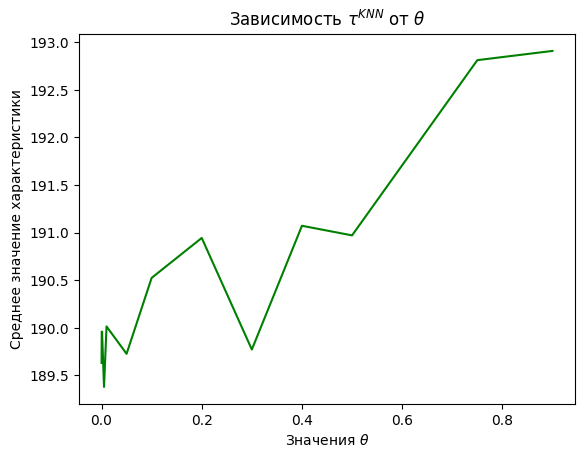
\includegraphics[width=0.5\linewidth]{1.png}
    \caption{LogNormal распределение с варьирующимся параметром $\theta$}
\end{figure}
\newline
\newline
При небольших $\theta$ среднее значение характеристики $\approx 190$ и начинает расти при $\theta \longrightarrow 1$.
\newline
\newline
Теперь посмотрим на $\theta \in [1, 500].$
\begin{figure}[h]
    \centering
    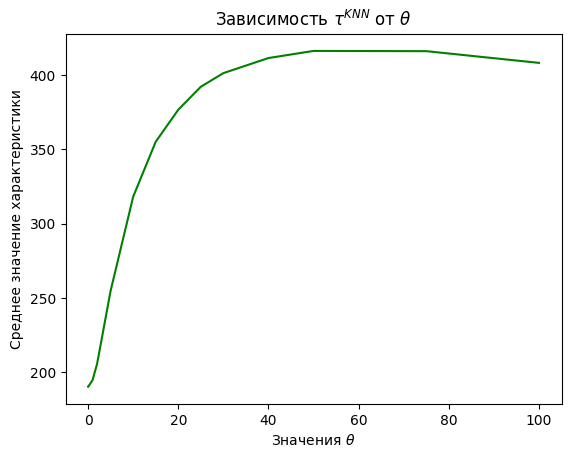
\includegraphics[width=0.5\linewidth]{2.png}
    \caption{LogNormal распределение с варьирующимся параметром $\theta$}
\end{figure}
\newline
\newline
При $\theta \in [1, 100]$ наблюдается резкий рост среднего значения характеристики, после этого кривая выравнивается и выходит на плато.

\subsection{Распределение Exp с параметром $\lambda$.}
Зафиксируем размер выборки $n = 50$ и количество соседей $k = 5$. Число итераций для метода Монте-Карло равно 1000.
\newline
\newline
Точно также будем перебирать $\nu \in (0, 1)$ и $\nu \in [1, 500]$.
\begin{figure}[h]
    \centering
    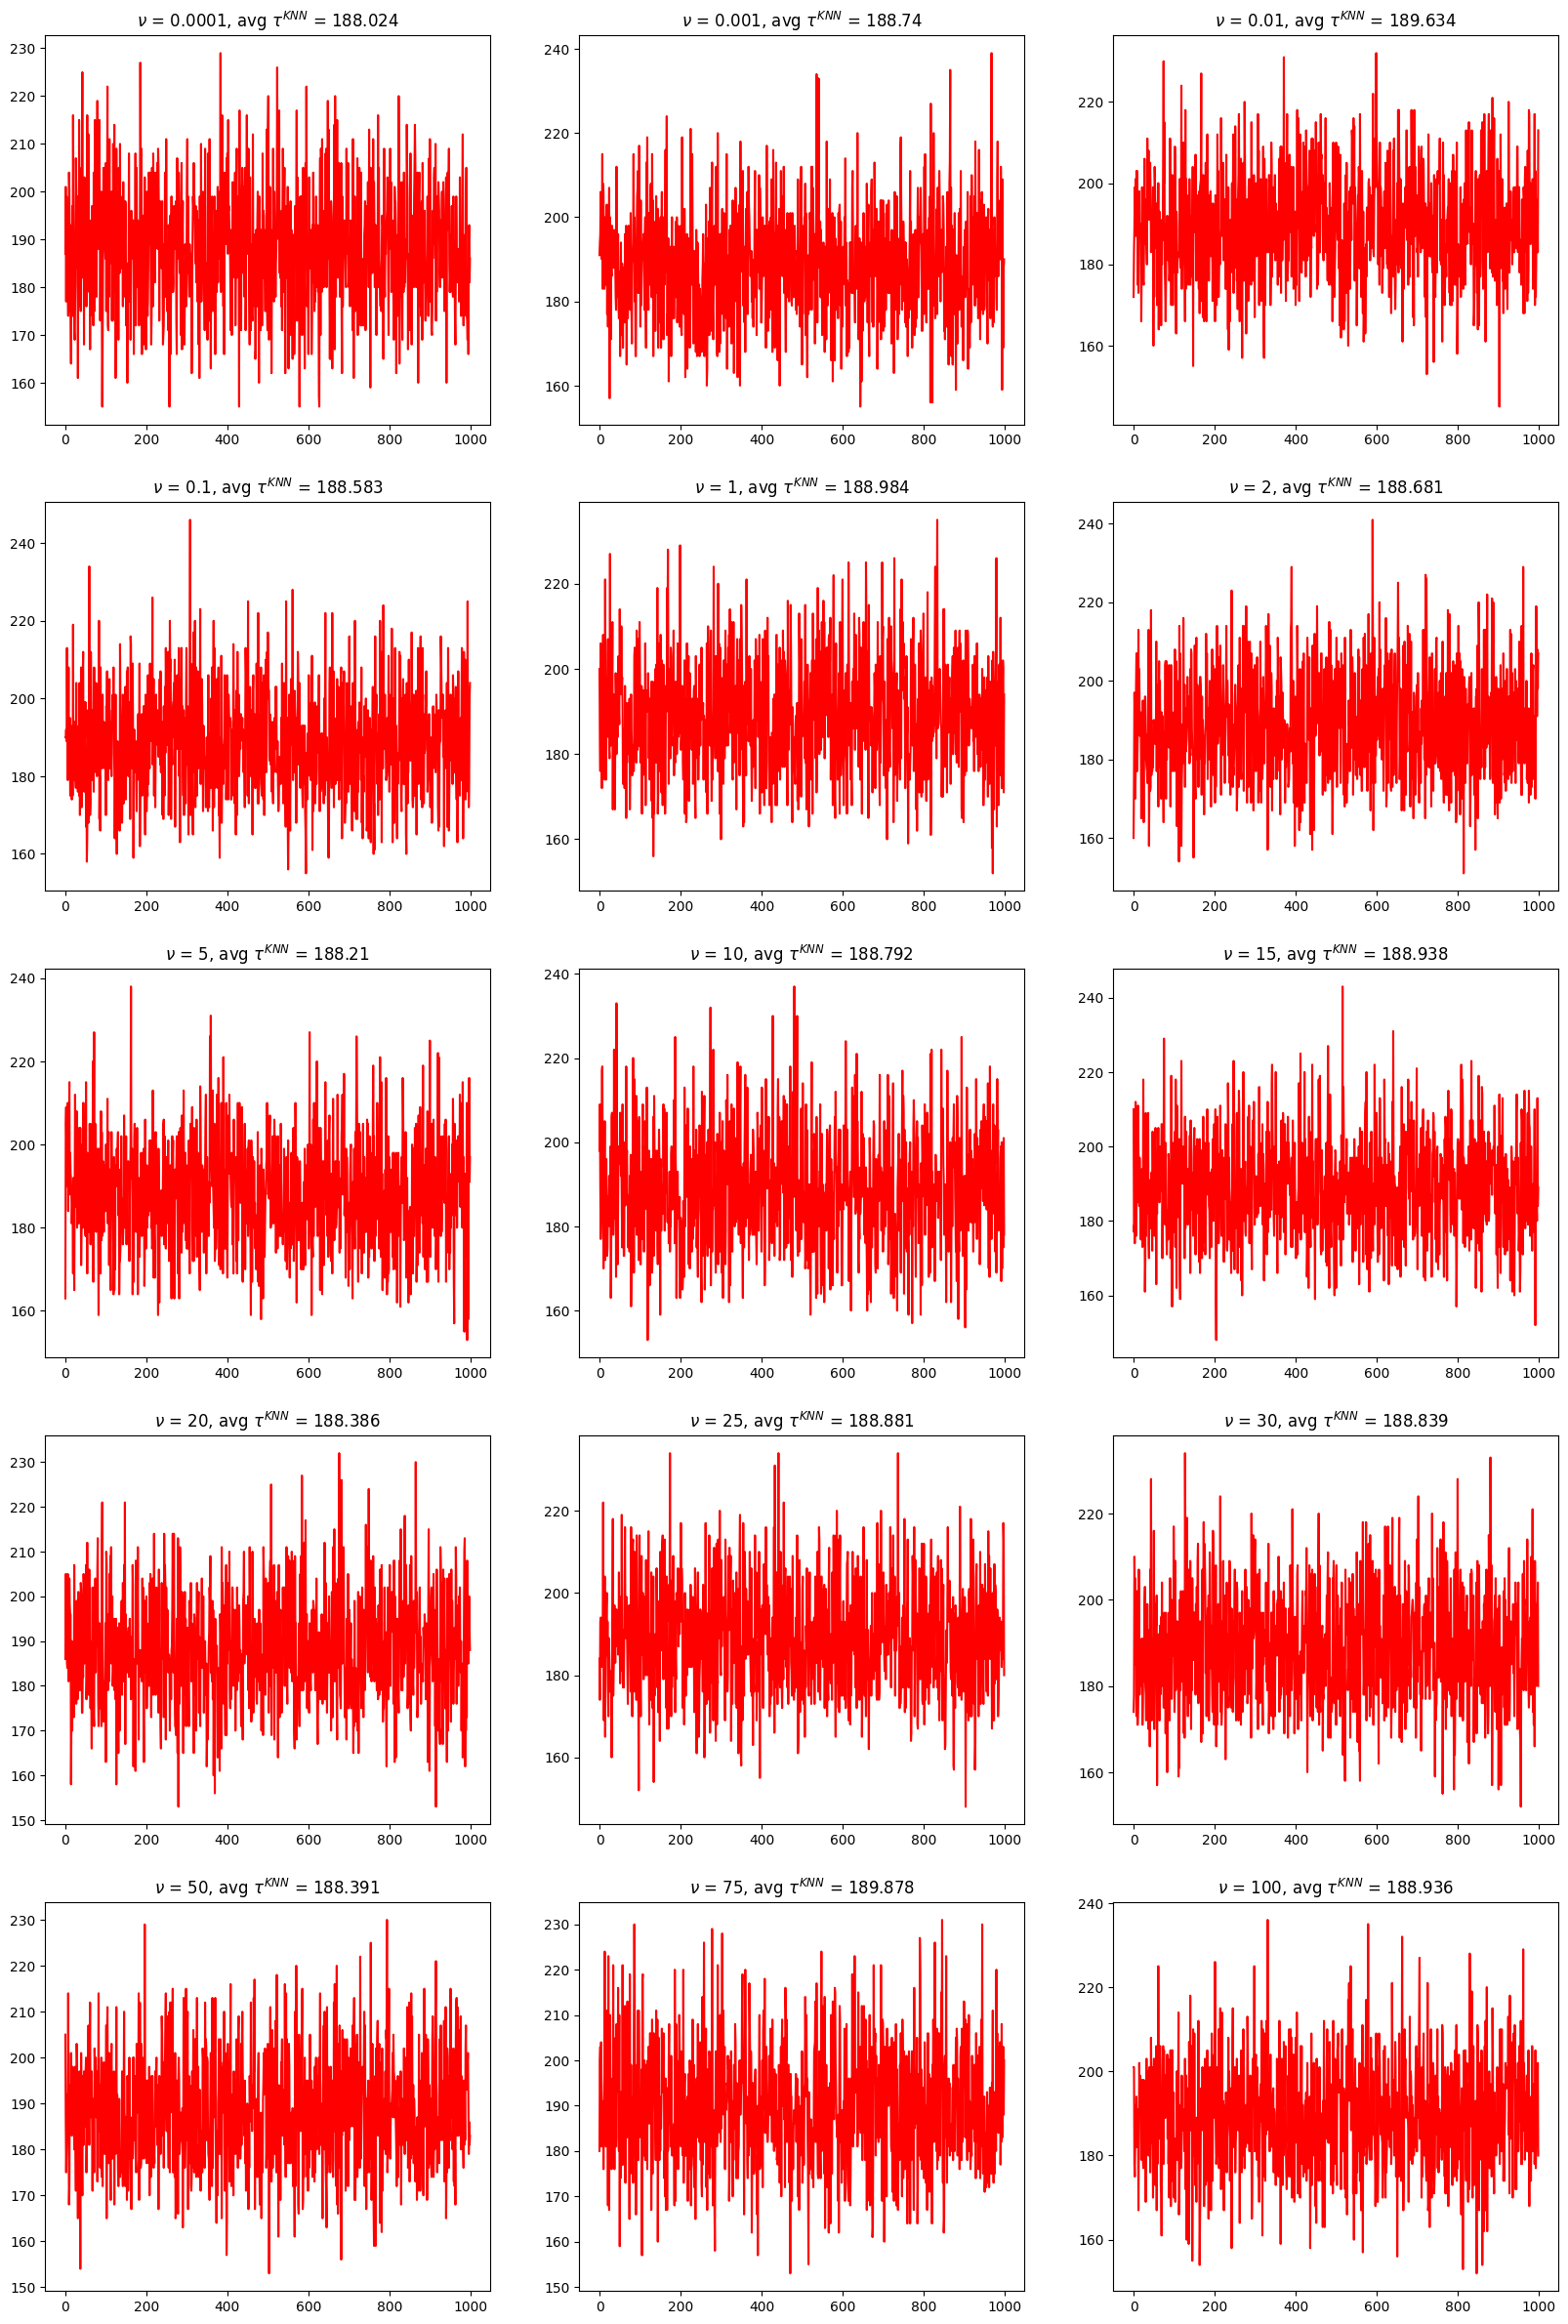
\includegraphics[width=0.5\linewidth]{3.png}
    \caption{Экспоненциальное распределение с варьирующимся параметром $\nu$}
\end{figure}
\begin{figure}[h]
    \centering
    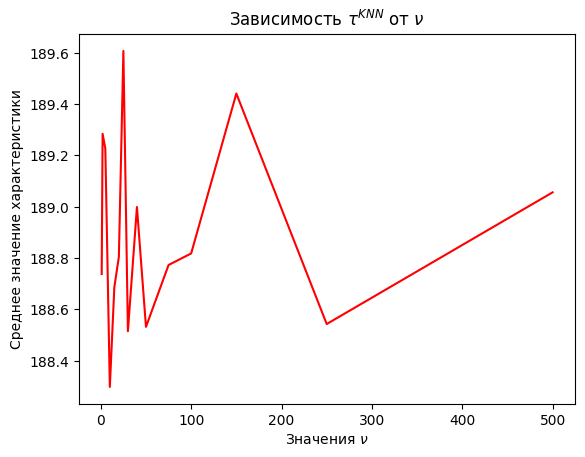
\includegraphics[width=0.5\linewidth]{4.png}
    \caption{Экспоненциальное распределение с варьирующимся параметром $\nu$}
\end{figure}
\newline
\newline
Усредненная характеристика $\tau^{KNN}$ принимает значения в окрестности числа 189 независимо от параметра $\nu$.

\subsection{Распределение SkewNormal с параметром $\alpha$.}
Зафиксируем размер выборки $n = 100$ и количество соседей $k = 5$. Число итераций для метода Монте-Карло равно 1000.
\newline
\newline
Будем перебирать $\theta = \{0.001, 0.01, 0.1, 0.5, 0.75, 1, 3, 5, 10, 15, 20, 50, 100, 500, 1000\}$.
\newline
\newline
\href{https://github.com/misshimichka/dm-random-graphs/blob/fbf3dd1bec269816312776019ca766ef0ce871b6/report/fix_construct_skewnorm_max_deg_knn.png}{Результаты}
\newline
\newline
Усредненная характеристика $\tau^{KNN}$ при любых значениях параметра $\tau$ приближенно равна 9, но при больших значениях это приближение становится более \href{https://github.com/misshimichka/dm-random-graphs/blob/dmitrii/report/report/fix_construct_skewnorm_alpha2avg_max_deg_knn.png}{заметным}. 

\subsection{Распределение Normal с параметром-дисперсией $\sigma$ и матожиданием 0.}
Зафиксируем размер выборки $n = 100$ и количество соседей $k = 5$. Число итераций для метода Монте-Карло равно 1000.
\newline
\newline
Будем перебирать $\nu = \{0.001, 0.01, 0.1, 0.5, 0.75, 1, 3, 5, 10, 15, 20, 50, 100, 500, 1000\}$.
\newline
\newline
\href{https://github.com/misshimichka/dm-random-graphs/blob/dmitrii/report/report/fix_construct_norm_max_deg_knn.png}{Результаты}
\newline
\newline
Усредненная характеристика $\tau^{KNN}$ принимает значения в окрестности числа 9 независимо от параметра $\nu$. Но при больших значениях параметра можно заметить \href{https://github.com/misshimichka/dm-random-graphs/blob/dmitrii/report/report/fix_construct_norm_sigma2avg_max_deg_knn.png}{здесь}, что характеристика $\tau^{KNN}$ начинает отклоняться от своего среднего значения.

\section{Характеристика $\tau^{dist}$.}
\subsection{Распределение LogNormal с $\mu$ = 0 и параметром $\theta$.}
Зафиксируем размер выборки $n = 50$ и расстояние $dist = 5$. Число итераций для метода Монте-Карло равно 1000.
\begin{figure}[h]
    \centering
    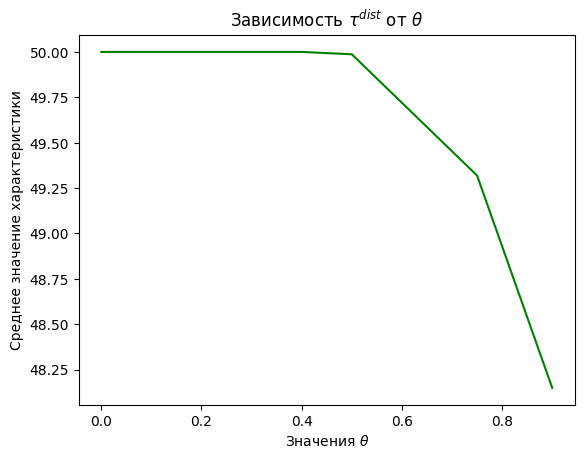
\includegraphics[width=0.5\linewidth]{5.png}
    \caption{LogNormal распределение с варьирующимся параметром $\theta$}
\end{figure}
\begin{figure}[h]
    \centering
    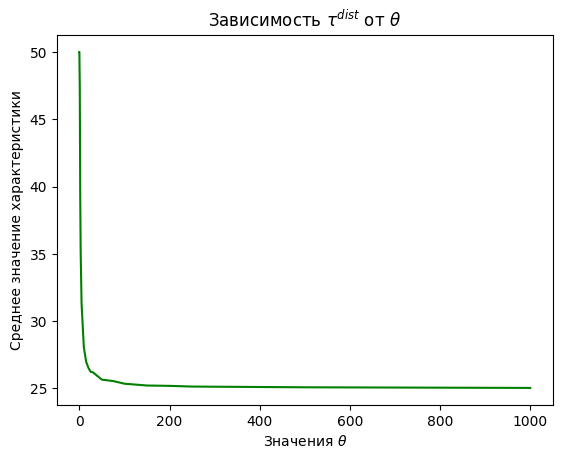
\includegraphics[width=0.5\linewidth]{6.png}
    \caption{LogNormal распределение с варьирующимся параметром $\theta$}
\end{figure}
\newline
\newline
С увеличением $\theta$ среднее значение характеристики $\tau^{dist}$ уменьшается, и при $\theta \approx 100$ принимает значение 25. Затем на больших $\theta$ среднее значение немного увеличивается и колеблется около 27.

\subsection{Распределение Exp с параметром $\lambda$.}
Зафиксируем размер выборки $n = 50$ и расстояние $dist = 5$. Число итераций для метода Монте-Карло равно 1000.
\begin{figure}[h]
    \centering
    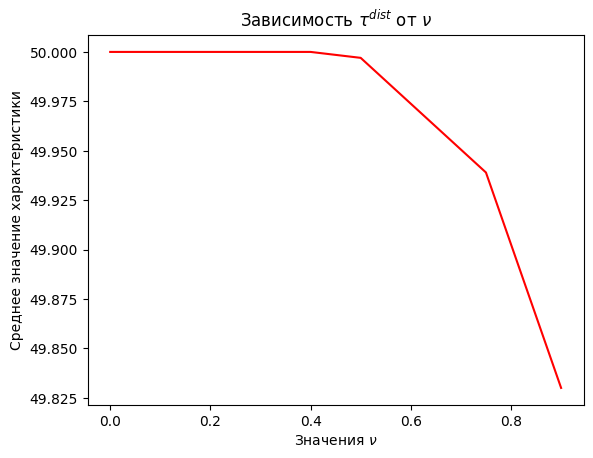
\includegraphics[width=0.5\linewidth]{7.png}
    \caption{Экспоненциальное распределение с варьирующимся параметром $\nu$}
\end{figure}
\begin{figure}[h]
    \centering
    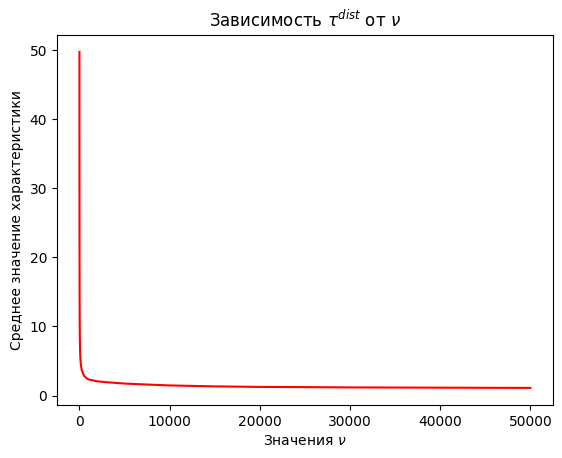
\includegraphics[width=0.5\linewidth]{8.png}
    \caption{Экспоненциальное распределение с варьирующимся параметром $\nu$}
\end{figure}
\newline
\newline
При больших $\nu$ среднее значение $\tau^{dist}$ стремится к 1.
\newline
\newline
Замечание: для экспоненциального распределения видно более резкое уменьшение значения характеристики по сравнению с lognormal распределением.

\subsection{Распределение SkewNormal с параметром $\alpha$.}
Зафиксируем размер выборки $n = 100$ и расстояние $dist = 1$. Число итераций для метода Монте-Карло равно 1000.
\newline
\newline
Будем перебирать \\
$\theta = \{0.001, 0.01, 0.1, 0.5, 0.75, 1, 3, 5, 10, 15, 20, 50, 100, 500, 1000, 10000, 150000, 300000, 500000, 15000000\}$.
\newline
\newline
\href{https://github.com/misshimichka/dm-random-graphs/blob/dmitrii/report/report/fix_construct_skewnorm_mis_dist.png}{Результаты}. 
\newline
\newline
Характеристика $\tau^{dist}$ при $\theta \in (0, 1)$ принимает в среднем значение 5, а при больших $\theta$ принимает значения, близкие к 3. Это хорошо видно на \href{https://github.com/misshimichka/dm-random-graphs/blob/dmitrii/report/report/fix_construct_skewnorm_alpha2avg_mis_dist.png}{графике}.

\subsection{Распределение Normal с параметром-дисперсией $\sigma$ и матожиданием 0.}
Зафиксируем размер выборки $n = 100$ и расстояние $dist = 5$. Число итераций для метода Монте-Карло равно 1000.
\newline
\newline
Будем перебирать \\
$\nu = \{0.001, 0.01, 0.1, 0.5, 0.75, 1, 3, 5, 10, 15, 20, 50, 100, 500, 1000, 10000, 150000, 300000, 500000, 15000000\}$
\newline
\newline
\href{https://github.com/misshimichka/dm-random-graphs/blob/dmitrii/report/report/fix_construct_norm_mis_dist.png}{Результаты}
\newline
\newline
Характеристика $\tau^{dist}$ при $\nu \in (0, 0.5)$ принимает значение 1 (т.е. при таких $\nu$ граф -- полный). С увеличением параметра растет среднее значение характеристики (можно посмотреть \href{https://github.com/misshimichka/dm-random-graphs/blob/dmitrii/report/report/fix_construct_norm_sigma2avg_mis_dist.png}{здесь}).

\chapter{Исследовать, как ведет себя числовая характеристика $\tau$ в зависимости от параметров процедуры построения графа и размера выборки при фиксированных значениях $\theta = \theta_0$ и $\nu = \nu_0$.}
[Тасина вставка] Сначала посмотрим на LogNormal и Exp распределения при данных $\theta_0$ и $\nu_0$:
\begin{figure}[h]
    \centering
    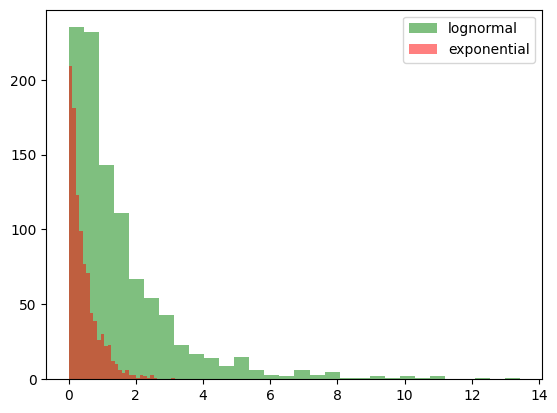
\includegraphics[width=0.5\linewidth]{distributions.png}
\end{figure}
\newline
\newline
Видно, что для построения дистанционного графа брать \texttt{dist} $> 5$ бессмысленно, т.к. при больших значениях \texttt{dist} число рёбер в графе стремится к $\binom{n}{2}$, где $n$ -- число вершин, соответственно, хроматическое число становится равным $n$ для обоих распределений.
\newline
\newline
Для нас же важно понимать, как различить между собой эти распределения, поэтому гораздо интереснее смотреть на графы с меньшим числом рёбер и смотреть на \texttt{dist} $\leq 5$.

\section{Характеристика $\tau^{KNN}$.}
\subsection{Распределение LogNormal с $\mu$ = 0 и $\theta = \theta_0 = 1$ и распределение Exp с параметром $\nu = \nu_0 = \frac{1}{\sqrt{e^2 - e}}$.}
Картинку смотрите тут: \texttt{\href{https://github.com/misshimichka/dm-random-graphs/blob/report/report/11.png}{11.png}}.
\newline
\newline
Замечания:
\newline
\newline
- $\tau^{KNN}$ для Exp распределения растет медленнее, чем для LogNormal распределения.
\newline
\newline
- При увеличении выборки разница между значениями характеристики для двух разных распределений растет. Это, конечно, хорошо, но computationally может быть неприятно. Хочется смотреть и на небольшую выборку, а в нашем случае разница между распределениями на небольших размерах почти не различима.
\newline

\subsection{Распределение SkewNormal с параметром $\alpha_0=1$.}
Будем перебирать параметры с 1000 итерациями метода Монтэ-Карло:\\
1. $n\_samples = \{[1, 5, 10, 25, 50, 100, 300]\}$\\
2. $k\_neighbours = \{1, 3, 5, 7, 9, 15, 20\}$

\href{https://github.com/misshimichka/dm-random-graphs/blob/dmitrii/report/report/fix_alpha_skewnorm_max_deg_knn.png}{Результаты}

Можно заметить, что средняя величина характеристики $\tau^{KNN}$ увеличивается, по мере роста перебираемых параметров. Но также часто встречаются ситуация, когда среднее значение совпадает с реальным.

\subsection{Распределение Normal с параметром-дисперсией $\sigma_0=1$ и матожиданием 0.}
Будем перебирать параметры с 1000 итерациями метода Монтэ-Карло:\\
1. $n\_samples = \{[1, 5, 10, 25, 50, 100, 300]\}$\\
2. $k\_neighbours = \{1, 3, 5, 7, 9, 15, 20\}$

\href{https://github.com/misshimichka/dm-random-graphs/blob/dmitrii/report/report/fix_sigma_norm_max_deg_knn.png}{Результаты}

Можем наблюдать такую же тенденцию -- с ростом параметров растет среднее значение характеристики, даже значения принимаются такие же со сдвигом на небольшой $\epsilon$.

\section{Характеристика $\tau^{dist}$.}
\subsection{Распределение LogNormal с $\mu$ = 0 и $\theta = \theta_0 = 1$ + распределение Exp с параметром $\nu = \nu_0 = \frac{1}{\sqrt{e^2 - e}}$.}
Картинку смотрите тут: \texttt{\href{https://github.com/misshimichka/dm-random-graphs/blob/report/report/14.png}{14.png}}.
\newline
\newline
Пара замечаний:
\newline
\newline
- $\tau^{dist}$ для Exp распределения растет быстрее, чем для LogNormal распределения.
\newline
\newline
- пока что $\tau^{dist}$ рассматривать и изучать приятнее/проще, чем $\tau^{KNN}$.

\subsection{Распределение SkewNormal с параметром $\alpha_0=1$.}
Будем перебирать параметры с 1000 итерациями метода Монтэ-Карло:\\
1. $n\_samples = \{[1, 5, 10, 25, 50, 100, 300]\}$\\
2. $dists = \{0.001, 0.01, 0.1, 0.5, 1, 3, 5\}$

\href{https://github.com/misshimichka/dm-random-graphs/blob/dmitrii/report/report/fix_alpha_skewnorm_mis_dist.png}{Результаты}

Можно заметить, что больше всего на значение характеристики $\tau^{dist}$ влияет параметр $n\_samples$, а с увеличением параметра $dist$ увеличивается количество ребер из-за этого уменьшается количество независимых вершин. 

\subsection{Распределение Normal с параметром-дисперсией $\sigma_0=1$ и матожиданием 0.}
Будем перебирать параметры с 1000 итерациями метода Монтэ-Карло:\\
1. $n\_samples = \{[1, 5, 10, 25, 50, 100, 300]\}$\\
2. $k\_neighbours = \{1, 3, 5, 7, 9, 15, 20\}$

\href{https://github.com/misshimichka/dm-random-graphs/blob/dmitrii/report/report/fix_sigma_norm_mis_dist.png}{Результаты}

Для каждого значения параметра $n\_samples$ можем заметить довольно плотное распределение среднего значения характеристики $\tau^{dist}$, но с ростом этого параметра растет количество выбросов и колебания.

\chapter{Построить множество A в предположении $\theta = \theta_0$ и $\nu = \nu_0$ при максимальной допустимой вероятности ошибки первого рода $\alpha = 0.05$. Оценить мощность полученного критерия.}
\section{Характеристика $\tau^{KNN}$.}
Для визуализаций смотрите картинку \texttt{\href{https://github.com/misshimichka/dm-random-graphs/blob/report/report/15.png}{15.png}}.
\newline
\newline
Распределения смешаны между собой, и трудно определить какую-либо границу между ними. Выходит, что работать с KNN-графом довольно неприятно. Посмотрим на дистанционный граф.

\section{Характеристика $\tau^{dist}$.}
Для визуализаций смотрите картинку \texttt{\href{https://github.com/misshimichka/dm-random-graphs/blob/report/report/16.png}{16.png}}.
\newline
\newline
А вот тут четко просматривается граница между двумя распределениями, особенно при бОльших размерах выборки. Построим множество $A$ (синие пунктирные линии на графике).
\newline
\newline
Посмотреть картинку можно тут: \texttt{\href{https://github.com/misshimichka/dm-random-graphs/blob/report/report/17.png}{17.png}}.
\newline
\newline
При увеличении $dist$ и размера выборки граница между двумя распределениями становится более явной. И даже есть примеры, когда мощность максимальна и равна 1.
Однако при небольших размерах выборки и маленьких $dist$ распределения довольно трудно различимы. В таких случаях и ошибка первого рода большая.
\newline
\newline
\emph{Вывод:} если дана выборка достаточного размера, то при выборе правильного $dist$ (кажется, что значения 2, 3, 5 подходят) можно построить дистанционный граф так, что по хроматическому числу этого графа будет возможно определить исходное распределение.

\part{Несколько характеристик проверки гипотезы.}
\chapter{Тасина часть}
Сгенерировала три набора данных для дистанционных графов:
\begin{itemize}
    \item 10000 значений характеристик для графов на 25 вершинах (по 5000 значений для каждого распределения).
    \item 10000 значений характеристик для графов на 100 вершинах (по 5000 значений для каждого распределения).
    \item 2000 значений характеристик для графов на 500 вершинах (по 1000 значений для каждого распределения). Размер меньше, чем у предыдущих двух наборов, т.к. для графов на 500 вершинах классификация довольно простая, и это видно еще из 1 части задачи по построению множества А.
\end{itemize}
Для дистанционных графов зафиксировала $dist = 1$, т.к. для больших значений решать задачу не очень интересно -- тогда граф становится все больше похож на полный. А при маленьких значениях многие характеристики для обоих распределений совпадают. Ну и судя по графикам из 1 части, именно выбранное значение $dist$ рассмотреть будет интересно, и в то же время не очень сложно.
\newline
\newline
Я использую следующие характеристики:
\begin{itemize}
    \item хроматическое число графа.
    \item число треугольников.
    \item максимальная степень вершины.
\end{itemize}
Размер максимального независимого множества не использую, т.к. он выражается через хроматическое число (при условии, что хроматическое число равно кликовому числу -- что верно в дистанционных графах): 
$$\alpha(G) = n - \chi(G),$$
где $n$ -- число вершин в графе. Соответственно, никакой новой информации эта характеристика не несет.
\newline
\newline
В качестве классификаторов я использую логистическую регрессию, дерево решений и случайный лес.

\section{Число вершин в графе = 25.}
Для графов на 25 вершинах лучше всего отработала логистическая регрессия. Возможно, это произошло, т.к. между характеристиками двух распределений граница не такая уж и заметная, поэтому эвристические алгоритмы (типа дерева решений или случайного леса) работали хуже. 
\newline
\newline
Если смотреть на ошибку первого рода, то она не превосходит $\alpha = 0.05$, т.е. все три классификатора подходят как статистические критерии.
\newline
\newline
При этом лучшим алгоритмом по мощности и по точности является логистическая регрессия.

\section{Число вершин в графе = 100.}
В этом случае результаты вообще прекрасные -- граница между характеристиками разных распределений стала более видимой, поэтому и точность стала выше.
\newline
\newline
И конечно, все три классификатора дают ошибку первого рода меньше, чем $\alpha = 0.05$.
\newline
\newline
Тут лучше всего отработали дерево решений и случайный лес.

\section{Число вершин в графе = 100.}
Тут, как и предполагалось, высокая точность при использовании всех алгоритмов, т.к. разделение между распределениями довольно четкое, и это было видно еще в 1 части задания.
\newline
\newline
Если смотреть на важность признаков, то довольно понятен алгоритм работы дерева решений: в основе его работы лежит отбор признаков через предикаты, и при взгляде на картинку выше становится понятно, что если использовать, например, такой предикат: [Хроматическое число $\leq$ 350], то классификация распределений уже будет оптимальной. Поэтому признак "хроматическое число" является самым важным для дерева решений (и, судя по значениям, единственным используемым).
\newline
\newline
В этом случае все алгоритмы показали ошибку первого рода = 0 и мощность = 1.

\section{Общий вывод по трем экспериментам.}
\begin{itemize}
    \item Для логистической регресии наиболее важными признаками являются хроматическое число и максимальная степень вершины.
    \item Для каждого набора данных дерево решений считало важным лишь 1 признак, и он был разным для разных наборов. Кажется, это обусловлено лишь особенностью задачи и данных (конкретнее: по большей части все зависит от числа вершин, на которых строим граф), другого разумного объяснения не придумала.
    \item Случайный лес -- ансамбль нескольких деревьев решений, поэтому все признаки относительно одинаковые по важности.
\end{itemize}
Но в общем и целом все получилось, точность высокая у всех алгоритмов!

\chapter{Часть Дмитрия}

\section{Исследование важности характеристик, как признаков классификации и изучение важности характеристик с ростом $n$.}

Для исследований в этой части генерировались наборы данных размера 1000 для значений $n = 10, 25, 50, 100, 150$.\\

Для подсчета характеристик использовался дистанционный граф с параметром $dist = 2$.\\

Используемые характеристики:
\begin{itemize}
    \item число треугольников.
    \item хроматическое число графа.
    \item максимальная степень вершины.
\end{itemize}
\newpage

\subsection{Распределение и корреляция признаков при $n = 10$}
\begin{figure}[h]
    \centering
    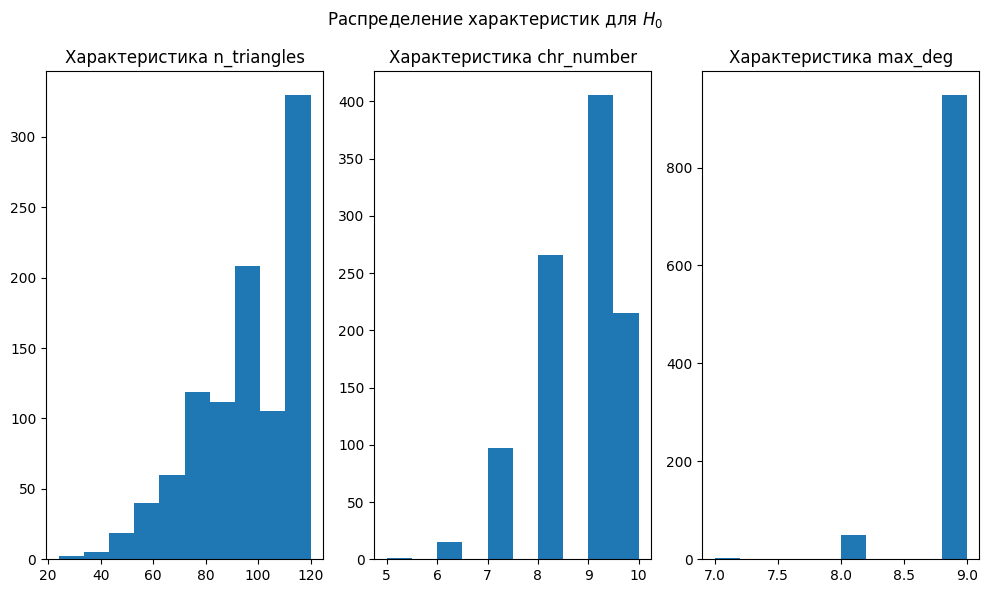
\includegraphics[width=0.4\linewidth]{n_10_h0_dist.png}
    \centering
    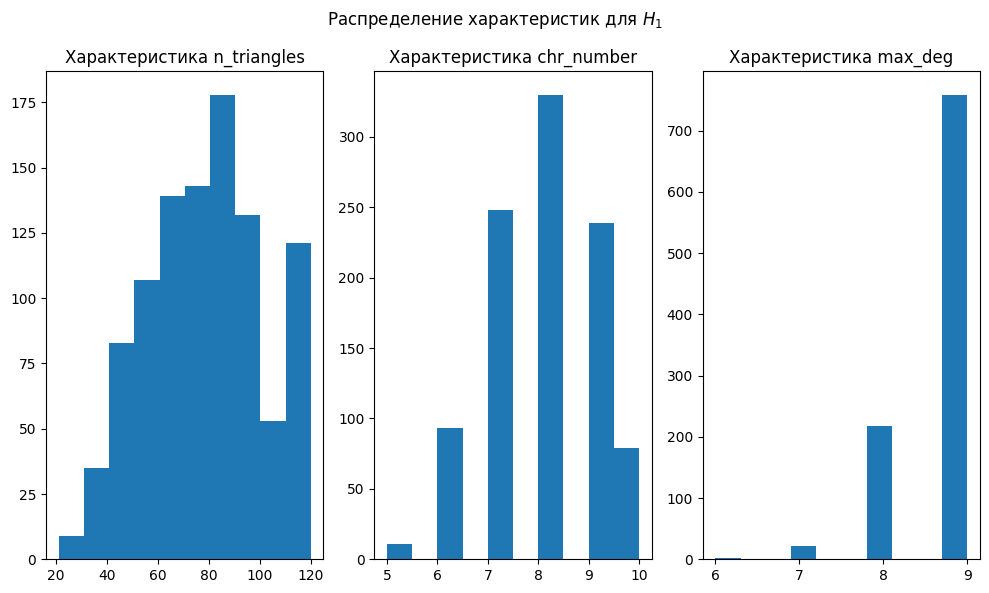
\includegraphics[width=0.4\linewidth]{n_10_h1_dist.png}
    \centering
    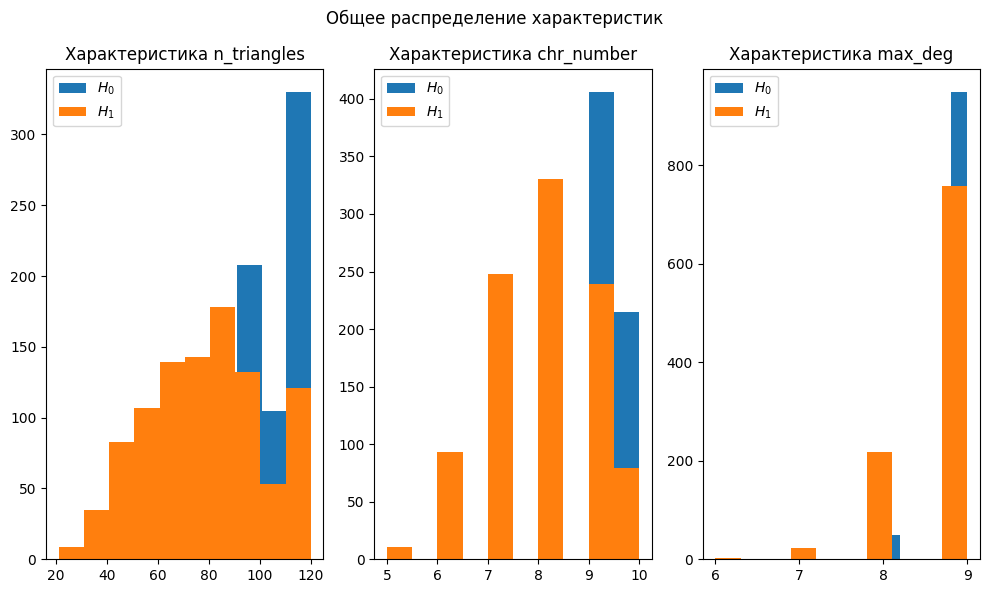
\includegraphics[width=0.4\linewidth]{n_10_common_dist.png}
\end{figure}

Как можем видеть, распределение характеристик почти не различимы, но некоторые особенности наблюдаются, например, значения характеристик для $H_0$ имеют большую частоту, это имеет смысл, ведь $H_0$ -- это сдвинутое нормальное распределение вправо, в дальнейших частях это смещение будет наблюдаться ещё сильнее.\\

Посмотрим на зависимость характеристик:
\begin{figure}[h]
    \centering
    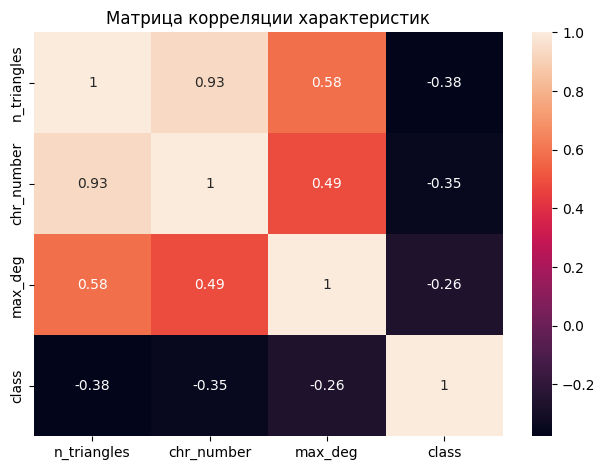
\includegraphics[width=0.4\linewidth]{n_10_corr.png}
    \centering
    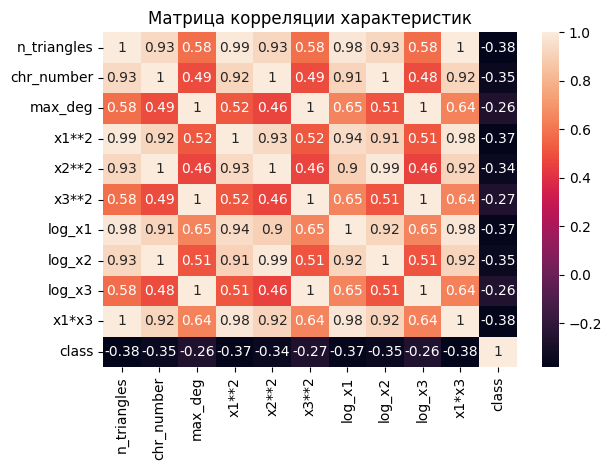
\includegraphics[width=0.4\linewidth]{n_10_extra_corr.png}
\end{figure}

Как можем заметить, все характеристики имеют высокую корреляцию между друг другом, а между целевым значением (гипотеза $H_0$ или $H_1$) наблюдается умеренная обратная корреляция, но самой коррелируемой характеристикой является число треугольников. Так же были рассмотрены дополнительные характеристики, но они повышения зависимости не дали.

\newpage
\subsection{Распределение и корреляция признаков при $n = 25$}
\begin{figure}[h]
    \centering
    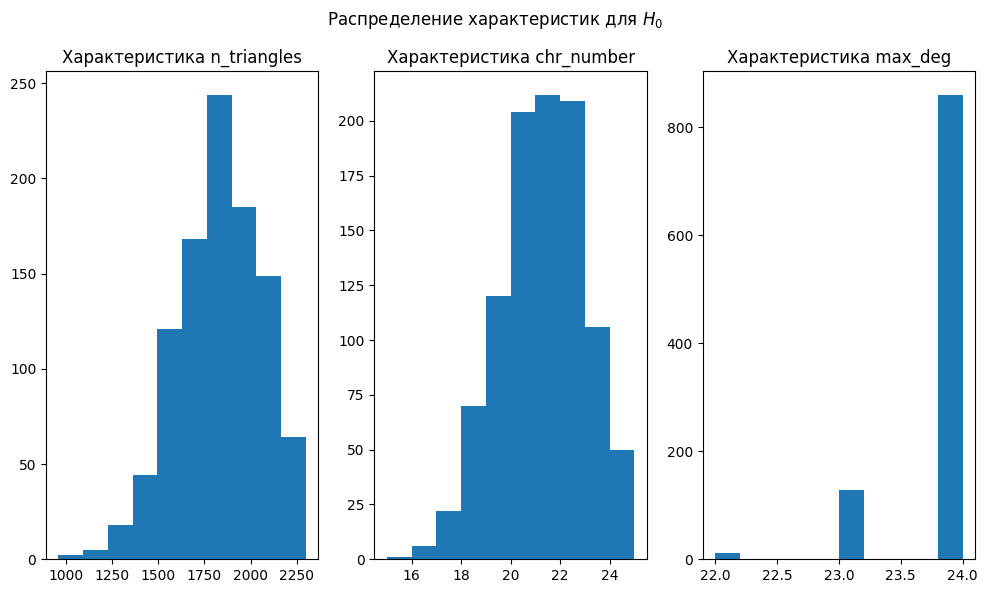
\includegraphics[width=0.4\linewidth]{n_25_h0_dist.png}
    \centering
    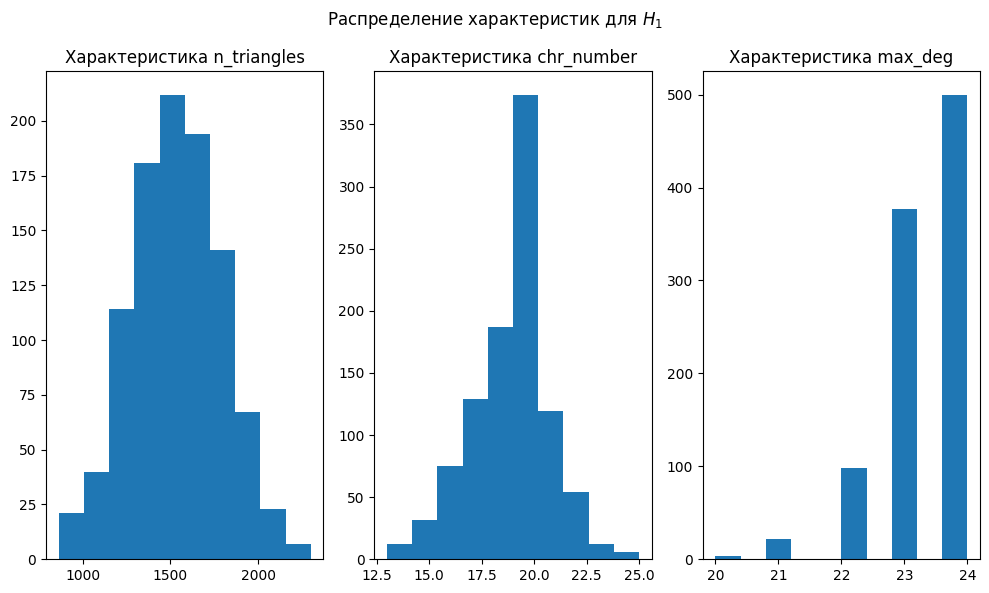
\includegraphics[width=0.4\linewidth]{n_25_h1_dist.png}
    \centering
    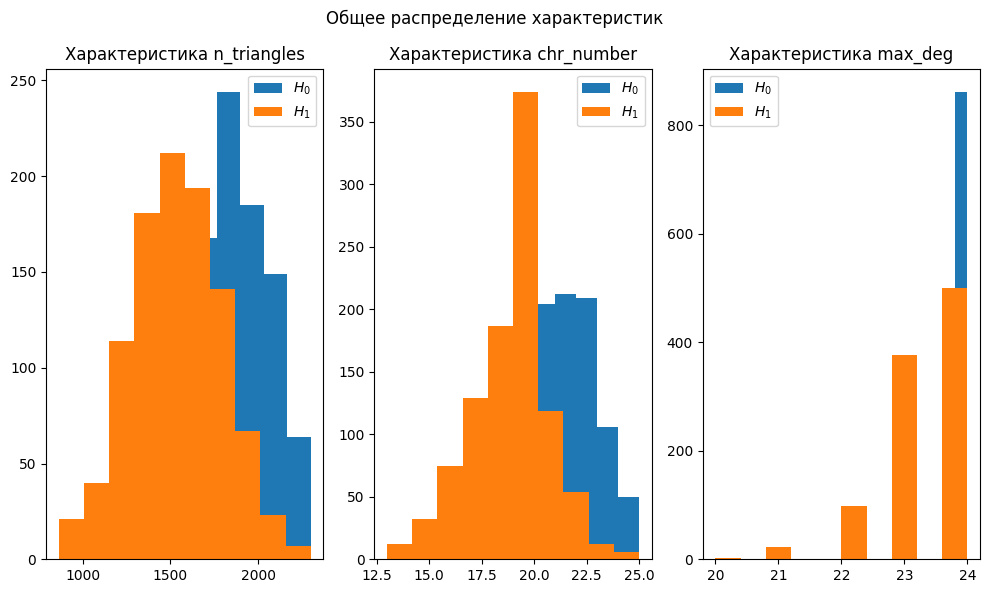
\includegraphics[width=0.4\linewidth]{n_25_common_dist.png}
\end{figure}

Здесь наблюдается ещё большее разделение значений, ещё большее смещение и рост значений.\\

Посмотрим на зависимость характеристик:
\begin{figure}[h]
    \centering
    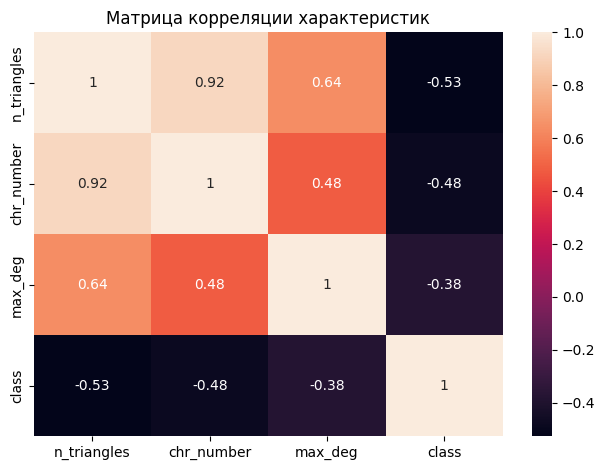
\includegraphics[width=0.4\linewidth]{n_25_corr.png}
    \centering
    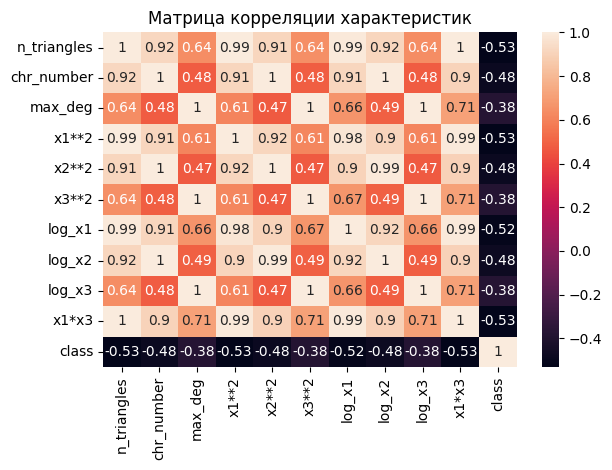
\includegraphics[width=0.4\linewidth]{n_25_extra_corr.png}
\end{figure}

Наблюдается рост зависимостей между характеристиками и целевым значением.

\newpage
\subsection{Распределение и корреляция признаков при $n = 50$}
\begin{figure}[h]
    \centering
    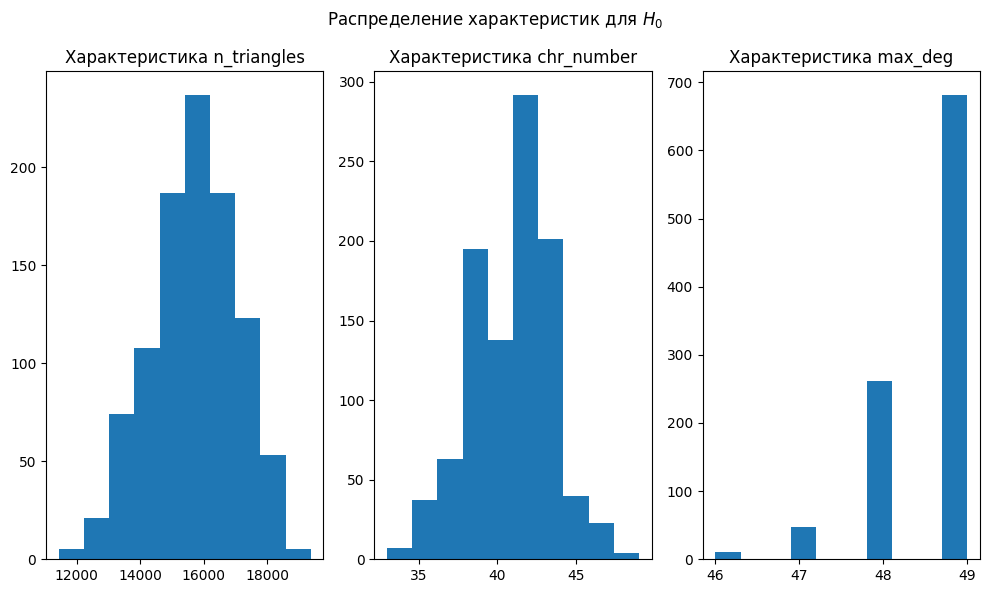
\includegraphics[width=0.4\linewidth]{n_50_h0_dist.png}
    \centering
    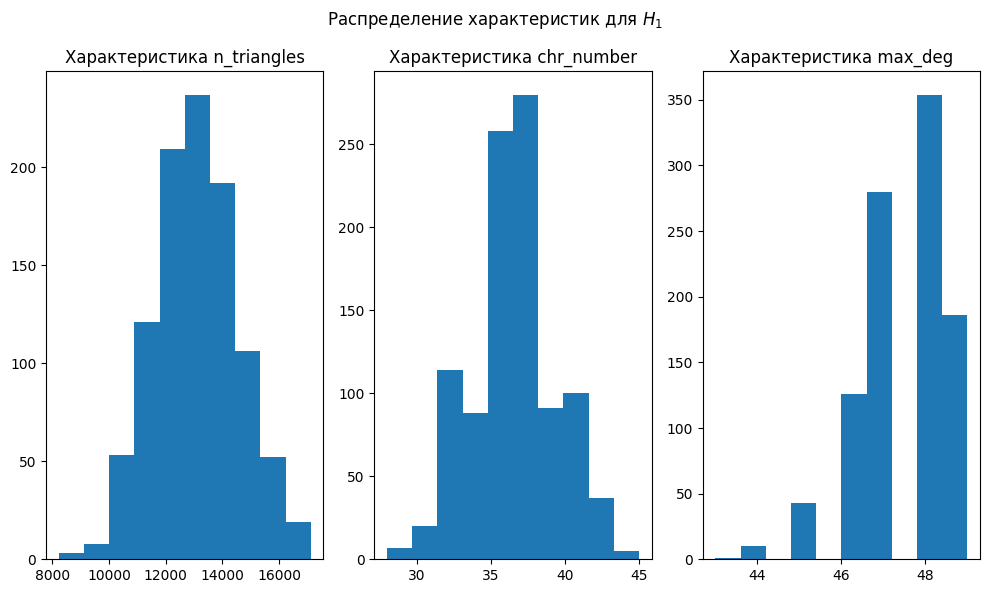
\includegraphics[width=0.4\linewidth]{n_50_h1_dist.png}
    \centering
    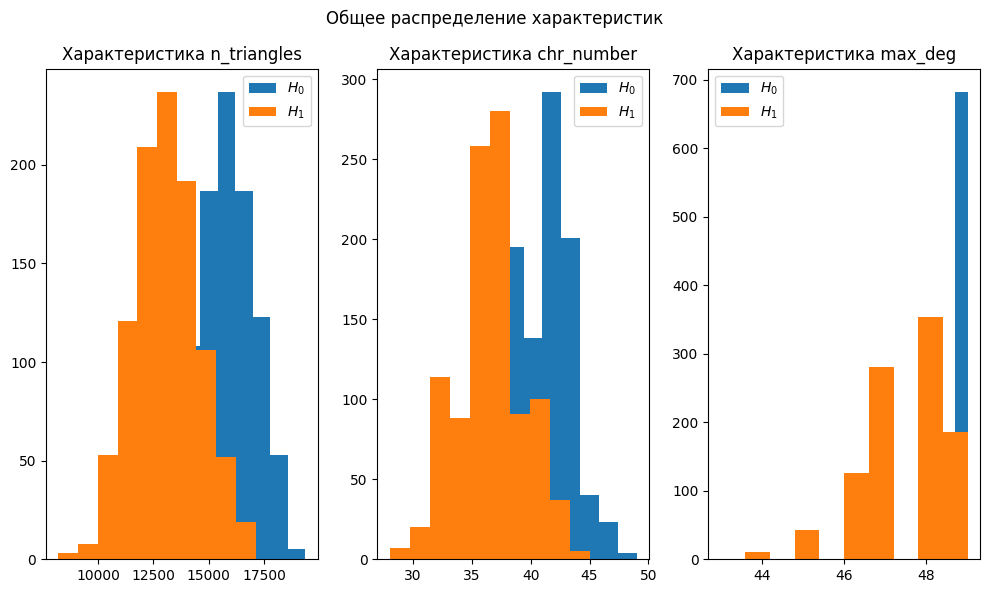
\includegraphics[width=0.4\linewidth]{n_50_common_dist.png}
\end{figure}\\

Посмотрим на зависимость характеристик:
\begin{figure}[h]
    \centering
    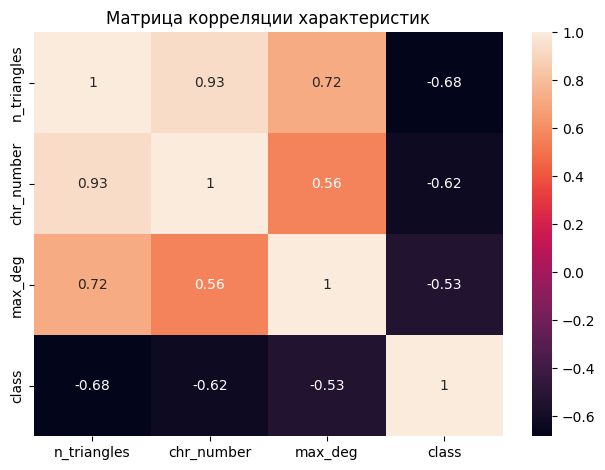
\includegraphics[width=0.4\linewidth]{n_50_corr.png}
    \centering
    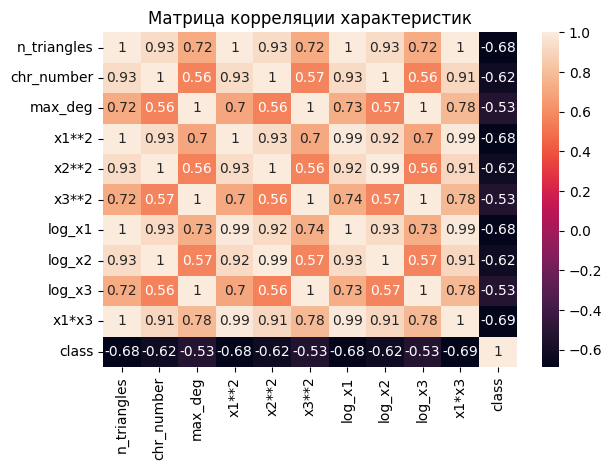
\includegraphics[width=0.4\linewidth]{n_50_extra_corr.png}
\end{figure}

\newpage
\subsection{Распределение и корреляция признаков при $n = 100$}
\begin{figure}[h]
    \centering
    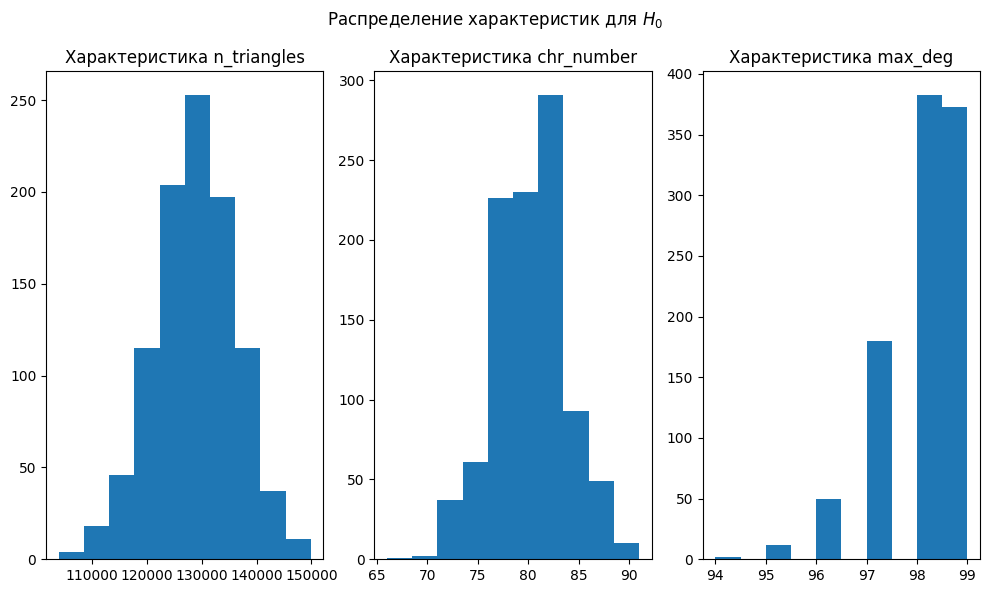
\includegraphics[width=0.4\linewidth]{n_100_h0_dist.png}
    \centering
    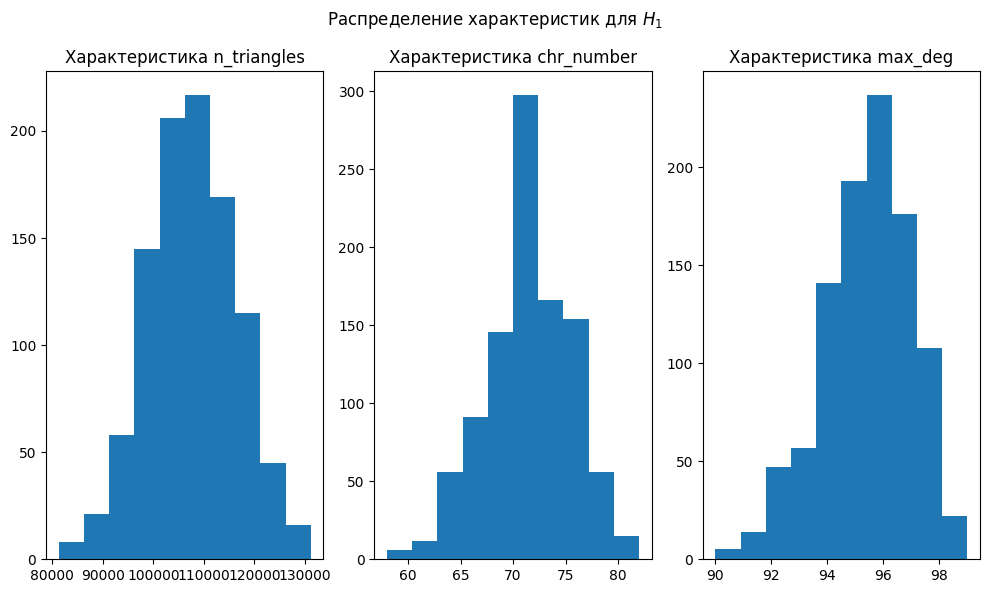
\includegraphics[width=0.4\linewidth]{n_100_h1_dist.png}
    \centering
    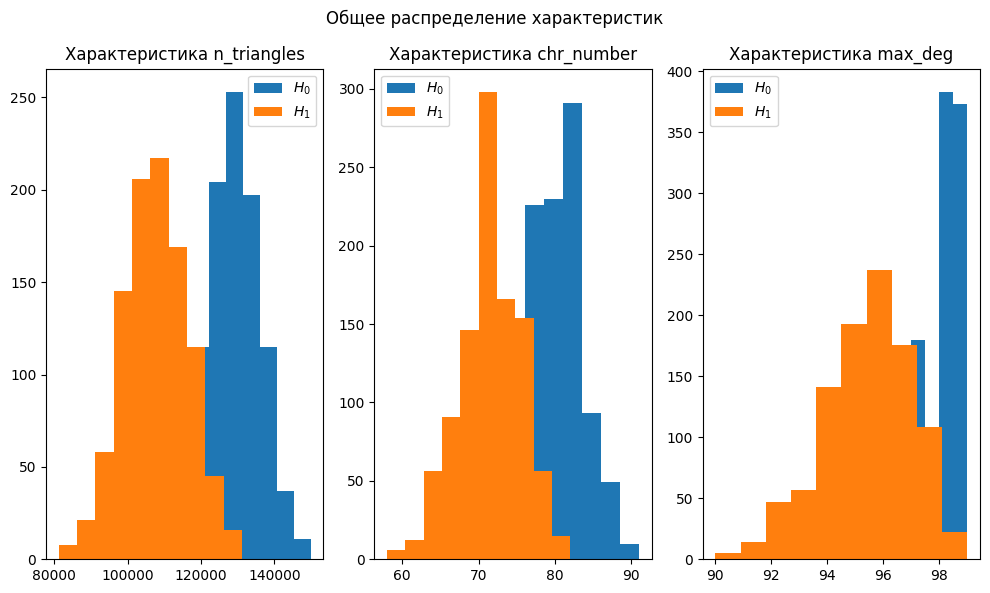
\includegraphics[width=0.4\linewidth]{n_100_common.png}
\end{figure}\\

Посмотрим на зависимость характеристик:
\begin{figure}[h]
    \centering
    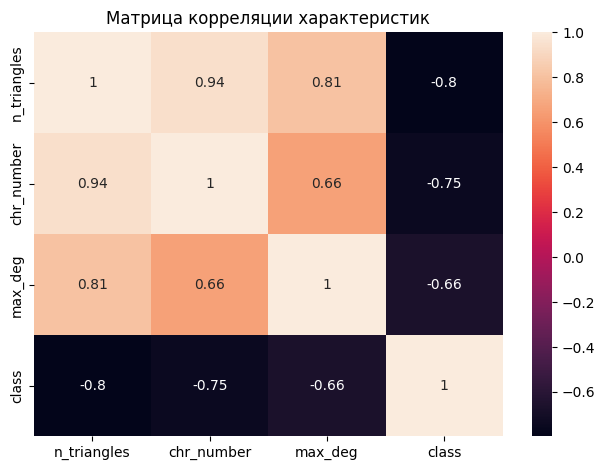
\includegraphics[width=0.4\linewidth]{n_100_corr.png}
    \centering
    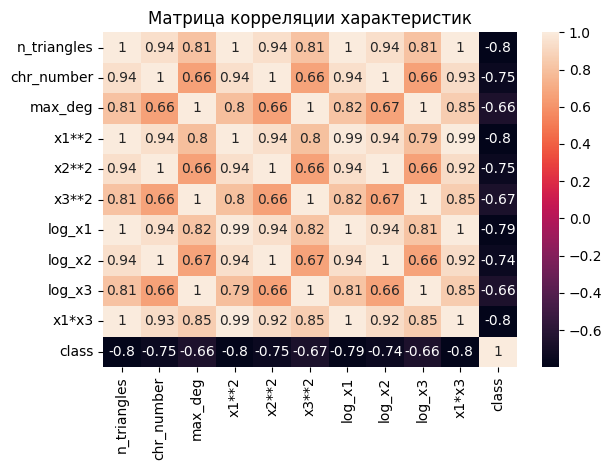
\includegraphics[width=0.4\linewidth]{n_100_extra_corr.png}
\end{figure}

\newpage
\subsection{Распределение и корреляция признаков при $n = 150$}
\begin{figure}[h]
    \centering
    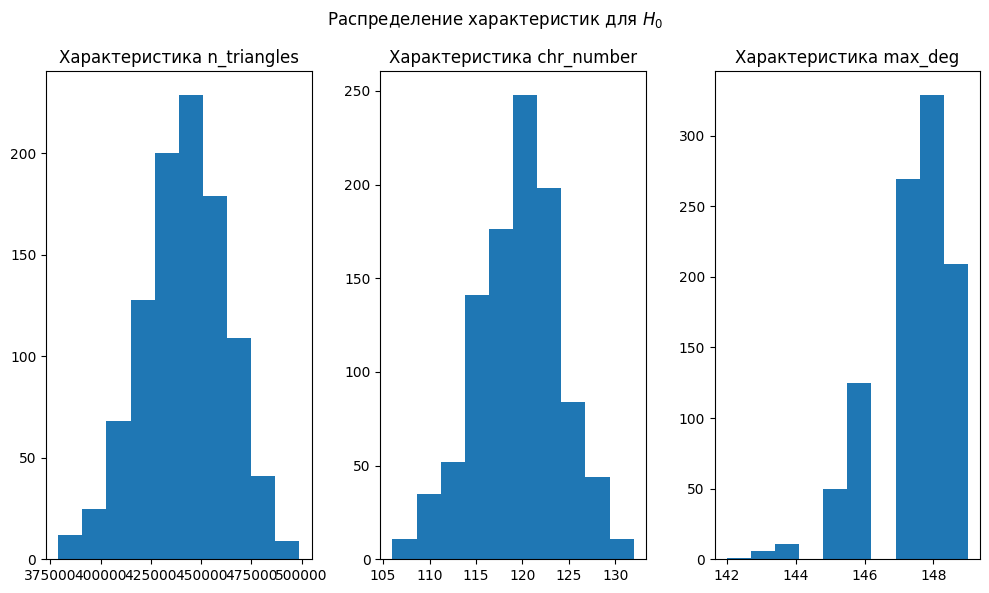
\includegraphics[width=0.4\linewidth]{n_150_h0_dist.png}
    \centering
    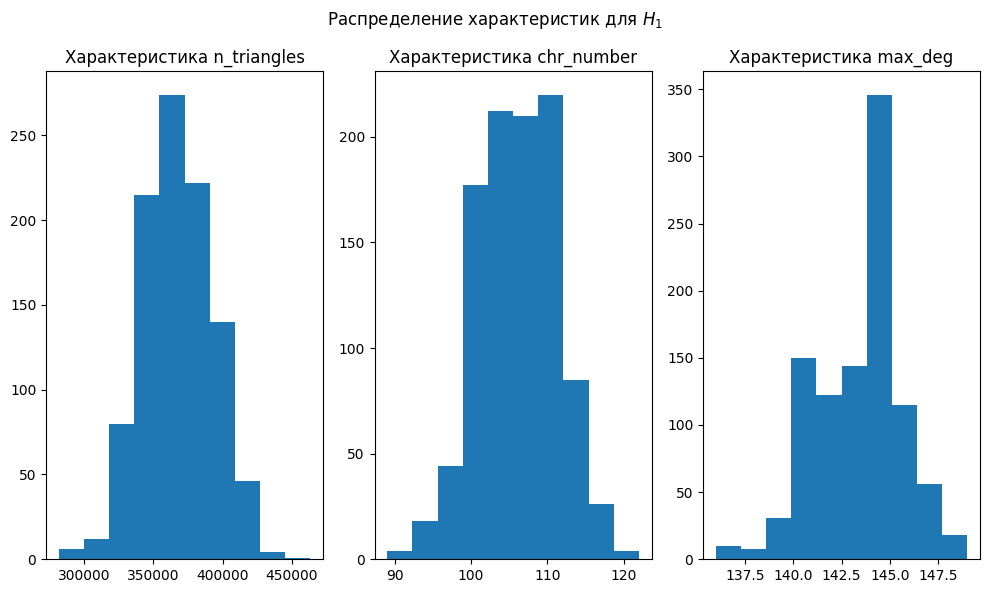
\includegraphics[width=0.4\linewidth]{n_150_h1_dist.png}
    \centering
    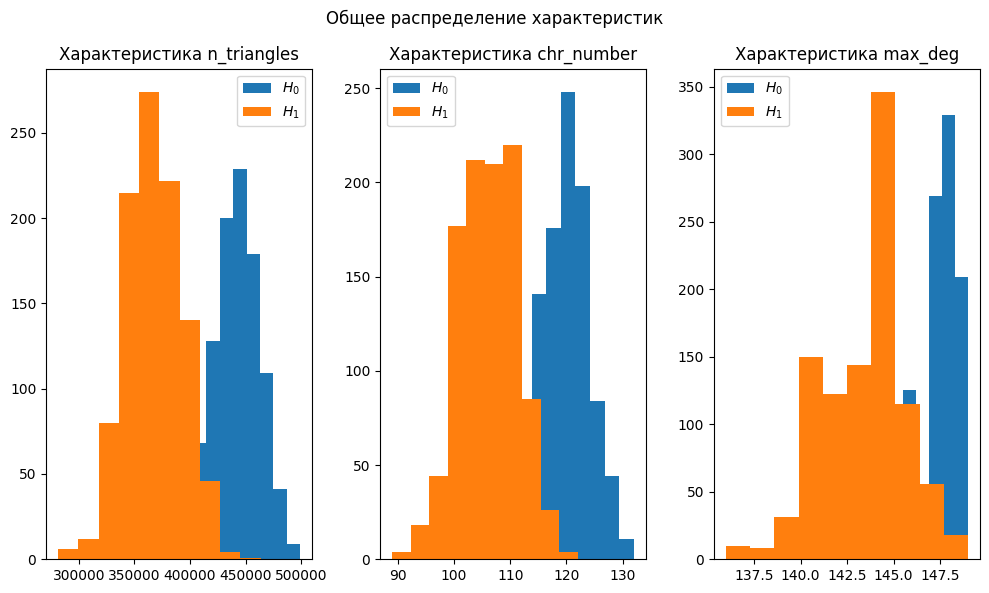
\includegraphics[width=0.4\linewidth]{n_150_common_dist.png}
\end{figure}\\

Можем наблюдать еще большее и очень заметное разделение значений.

Посмотрим на зависимость характеристик:
\begin{figure}[h]
    \centering
    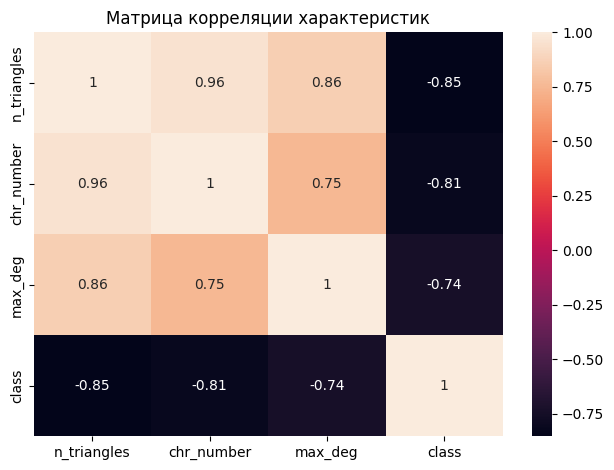
\includegraphics[width=0.4\linewidth]{n_150_corr.png}
    \centering
    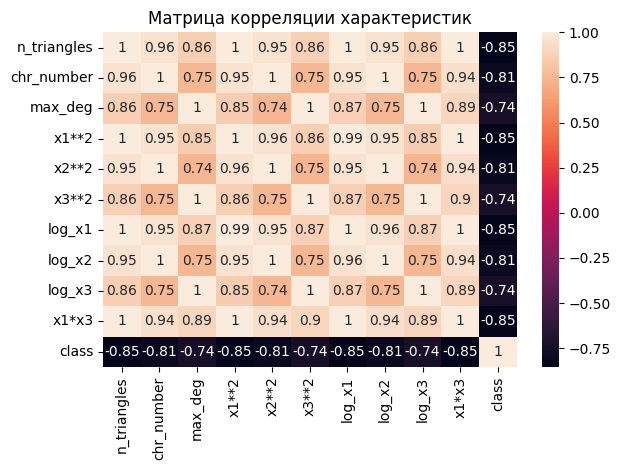
\includegraphics[width=0.4\linewidth]{n_150_extra_corr.png}
\end{figure}

Можем наблюдать высокую обратную корреляция между характеристиками и целевым значением.\\

В итоге можем заметить, что с ростом размера выборки растет корреляция между характеристиками и целевым значением, и разделение между значениями, которые соответствуют разным гипотезам, становится заметнее.
\newpage
\section{Применение классификационных алгоритмов.}

Определение гипотез можно рассмотреть как задачу классификации, а с этой задачей хорошо справляются ML-алгоритмы. 

Предлагаю рассмотреть алгоритмы:
\begin{itemize}
    \item $k$ ближайших соседей
    \item Логистическая регерессия
    \item Категориальный бустинг на решающих деревьях
\end{itemize}

Рассматриваемые метрики для задачи классификации:
\begin{itemize}
    \item $Accuracy$
    \item $Precision$
    \item $Recall$
    \item $f1-score$
\end{itemize}

Посмотрим на дисперсию метрик в зависимости от размера выборки:
\begin{figure}[h]
    \centering
    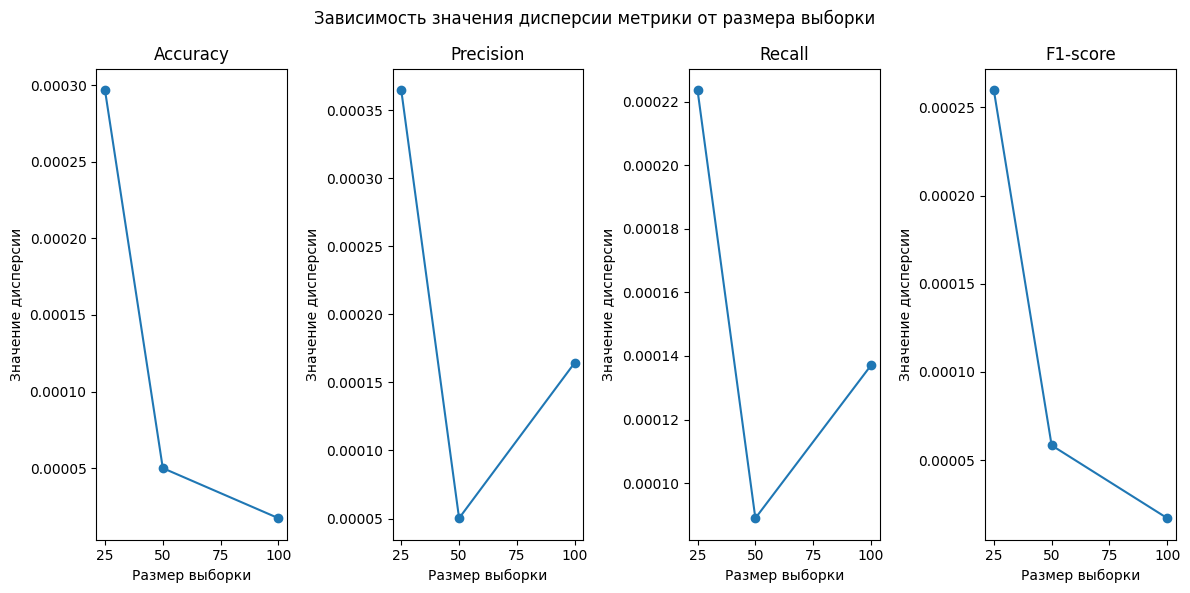
\includegraphics[width=0.5\linewidth]{metrics_var.png}
\end{figure}

Можем наблюдать, что с ростом размера выборки разброс значений метрик уменьшается.

Посмотрим на важность признаков для каждого классификатора:
\begin{figure}[h]
    \centering
    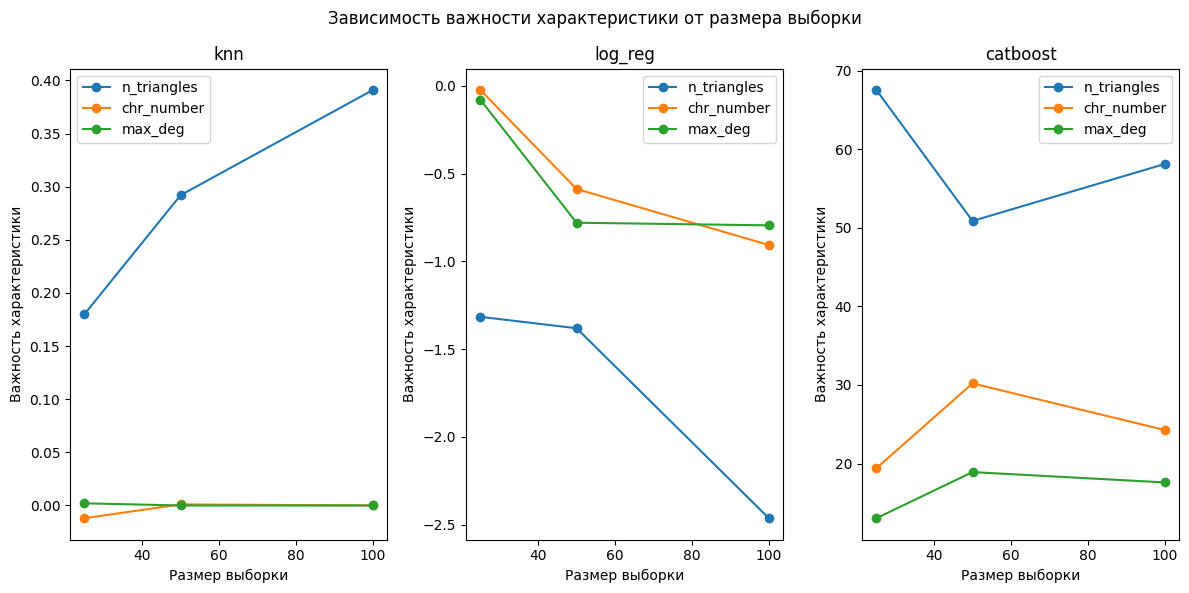
\includegraphics[width=0.5\linewidth]{char_imp.png}
\end{figure}

Можем наблюдать, что абсолютно самым важным признаком для всех классификаторов является число треугольников. Действительно, из секции выше заметно, что разделение значений наиболее заметно именно на этой характеристике.

\section{Вычисление ошибки первого рода, мощности и вывод}

Для подсчета ошибки первого рода и мощности будет использована логистическая регрессия, т.к. она показала самую высокую точность предсказаний.

Для случайного набора данных получим такие значения:
\begin{itemize}
    \item Ошибка первого рода $= 0.098$
    \item Мощность $= 0.906$
\end{itemize}

В итоге получили, что с ростом размера выборки, точность растет.

\end{document}